%2038
\newpage
\subsection{例題4-11 ゲームのタイトル画面を改造してみよう}


\begin{description}
    \item \textgt{\bf  考え方}
\end{description}


ジャンプアップゲーム(jump.hsp)のプログラムを改造して、タイトル画面を自分だけのものにしてみましょう。

\begin{figure}[H]
    \begin{center}
      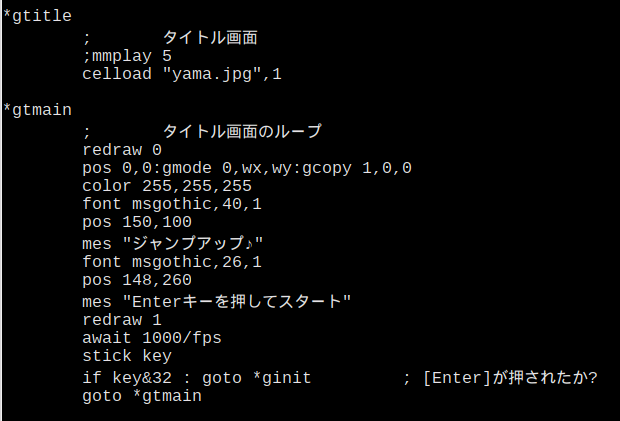
\includegraphics[keepaspectratio,width=14.42cm,height=9.791cm]{text04-img/text04-img033.png}
    \end{center}
    \label{fig:prog_menu}
\end{figure}


\begin{description}
    \item \textgt{\bf  例題4-11 答え}
\end{description}

背景の画像に「yama.jpg」、後は決められたサイズと色で文字を出しています。

「ジャンプアップ」ではない、別なタイトルを考えてみましょう。

どんな画面にしたいか、考えてから改造を始めましょう。

改造ができたらTAや周りの友達にも見せてあげましょう。



% Last Part:

%2083